\documentclass[conference]{IEEEtran}
\IEEEoverridecommandlockouts
\usepackage{cite}
\usepackage{amsmath,amssymb,amsfonts}
\usepackage{algorithmic}
\usepackage{graphicx}
\usepackage{textcomp}
\usepackage{xcolor}
\usepackage{tikz}
\usetikzlibrary{arrows.meta, positioning, calc, decorations.pathreplacing}
\graphicspath{{figures/}}

\def\BibTeX{{\rm B\kern-.05em{\sc i\kern-.025em b}\kern-.08em
    T\kern-.1667em\lower.7ex\hbox{E}\kern-.125emX}}

\begin{document}

\title{When Does Adaptive Recovery Pay?\\
A Failure-Aware Bandit Study of Recovery-Strategy\\
Selection in Autonomous LLM Agents}

\author{
\IEEEauthorblockN{Pio Micheal}
\IEEEauthorblockA{
Department of Artificial Intelligence and Data Science\\
Karunya Institute of Technology and Sciences\\
Coimbatore, India\\
Email: piomicheal17@gmail.com}
}

\maketitle

\begin{abstract}
Autonomous agents that call external tools fail in recurring, classifiable
ways, and recovery is increasingly treated as a decision problem rather
than a fixed exception handler. When the recovery choice is learned
online, a practical question follows: at what horizon does a learner
overtake a competent hand-written rule table? A predictor already in our
framework answers this, but only if the policy observes the true failure
type. Ours does not; every policy here acts on a classifier's predicted
type instead. We extend the predictor to the noisy-classifier case by
re-expressing the strategy-success matrix in predicted-type space through
an exact Bayes mixture, and split the resulting degradation into a
reward-ceiling piece and a learnability piece. At our trained classifier's
measured accuracy (0.939 mean diagonal), ceiling loss dominates
learnability loss roughly six to one. By construction, we also show the
predicted crossover horizon is not monotonic in classifier accuracy, even
though the static-side regret rate is. The extension's one free constant
was evaluated under a protocol registered before the supporting data
existed: an 18/8 train/test split, a transfer branch and an in-condition
branch, and a threshold fixed in advance. The observed ratio of held-out
errors, $R=1.4729$, clears the pre-committed threshold of 1.5, but the
same protocol's bootstrap interval, $[1.00, 9.55]$, does not confirm that
clearance is robust. We report the result as partially supported and
describe the extension as a calibrated predictor rather than a validated
bound. A companion investigation asks whether a low-dimensional statistic
predicts the sign of adaptive advantage under drift; this comes back
negative. Three pre-registered candidates were tried, one was retracted
for conceptual circularity, and none survives leave-one-cell-out
evaluation, though one qualitative finding does hold up: the sign is
governed by whether staleness damage reverts, not by how large it is.
\end{abstract}

\begin{IEEEkeywords}
autonomous agents, failure recovery, multi-armed bandits, Thompson
sampling, regret analysis, classifier noise, pre-registration, negative
results, reproducibility
\end{IEEEkeywords}

\section{Introduction}

Tool-using language agents fail often enough that handling failure is a
first-class design concern, not an edge case. Timeouts, tool exceptions,
malformed outputs, and lost context show up as the dominant failure modes
in deployed and benchmarked systems alike \cite{cemri2025,zhu2025,vuddanti2025}.
The usual response is a fixed mapping, $\pi(t)$, from failure type to
recovery strategy. That table is cheap and interpretable, and it can be
quite good, but it never improves; it is only as good as the designer's
beliefs on the day it was written.

An alternative treats each (failure type, recovery strategy) pair as a
bandit arm and learns its value from outcomes. This buys adaptation at
the price of exploration. Early on the learner is worse than a good
table, because it is still paying to find out what works, so whether
adaptation is worth it depends on the deployment horizon. A designer
choosing between the two wants an estimate of where the crossover falls.

An earlier part of this project, which we call the base predictor,
supplies exactly that estimate. It computes a static table's constant
per-episode regret rate exactly, models the learner's cumulative regret
with an asymptotic bound in the tradition of Lai and Robbins
\cite{lai1985}, and solves for the horizon where the two curves cross.
That construction assumes the policy sees the true failure type. Our
system does not give it one. We traced the call chain from the episode
loop through the adapter and selector layers into the matrix environment
and confirmed that no policy in the codebase has access to a true type;
the context object simply carries no field it could be read from. Every
policy here acts on a classifier's prediction. That is a structural fact
about the simulator, not a design choice, and it meant the base predictor
had been answering a question about a system we do not actually have.

This paper works through two extensions of the base predictor and
reports what happened to each. The contributions are:

\begin{enumerate}
\setlength\itemsep{1pt}
\setlength\parskip{0pt}
\item An exact reformulation of the crossover problem under an arbitrary
classifier confusion matrix, via Bayes' rule mapping the
success-probability matrix into predicted-type space. It reduces exactly
to the base predictor at a perfect classifier, and we separate which
pieces stay exact from which inherit the base predictor's asymptotic
approximation.
\item A decomposition of classifier-induced degradation into
reward-ceiling loss and gap shrinkage, measured at our trained
classifier's empirical confusion matrix, plus a construction showing the
predicted crossover horizon is not monotonic in classifier accuracy.
\item A pre-registered, environment-level held-out evaluation of the
extension's free constant on a 26-environment dataset generated after the
protocol was committed, including the uncertainty quantification the
protocol required, which keeps the result from reading as strong
confirmation.
\item A documented negative result on whether the sign of adaptive
advantage under drift reduces to a low-dimensional statistic, including a
retracted attempt and one qualitative finding that survives.
\item Measurement findings on cost estimation for long parallel sweeps
that invalidate the linear-speedup assumption behind our own previously
published cost figures.
\end{enumerate}

To be clear about what is not claimed: the extension does not make the
underlying asymptotic bound accurate, held-out absolute errors stay large
at roughly 40--60\%. The evaluation only tests whether the
classifier-noise reformulation adds model error on top of what the base
bound already carries, and even that rests on a point estimate with a
wide interval.

\section{Background and Related Work}

Recent work has moved from anecdotal failure reports toward structured
taxonomies. Cemri et al. derive an empirically grounded taxonomy of
multi-agent failure modes spanning system design, inter-agent
misalignment, and task verification \cite{cemri2025}. Zhu et al. take a
single-agent, module-oriented view, attributing failures to memory,
reflection, planning, action, and system-level operations, with a
debugging framework that isolates the earliest error whose correction
changes the outcome \cite{zhu2025}. Song et al. study the complementary
problem of optimising the environment rather than the agent, with their
own taxonomy of agent-environment interaction failures
\cite{song2025aegis}. On the response side, Reflexion has agents
verbalise reflections on failed attempts into an episodic buffer
\cite{shinn2023}, CRITIC has the model consult external tools to verify
and revise its own outputs \cite{gou2024}, and PALADIN trains recovery
behaviour directly from systematically injected tool failures
\cite{vuddanti2025}.

The framework this paper extends sits somewhere else. It is not proposing
a new self-correction mechanism. It asks how a recovery-strategy selector
should be evaluated against a static baseline, treating selection as a
bandit problem with persistent outcome memory. This paper narrows that
further still, to the analytic prediction of when a selector overtakes
its baseline, and what happens to that prediction once the failure type
fed to the selector is itself noisy.

Failures are drawn from seven types and recovered with one of six
strategies (\texttt{retry}, \texttt{replan}, \texttt{switch\_tool},
\texttt{re\_ground}, \texttt{verify}, \texttt{clarify}), giving $N=7$ and
$K=6$ throughout this paper. The seven types are largely self-descriptive
by name: \texttt{tool\_timeout}, \texttt{tool\_error},
\texttt{wrong\_tool\_selected}, \texttt{hallucinated\_output},
\texttt{malformed\_output}, \texttt{context\_loss}, and
\texttt{ambiguous\_instruction}.

The exploration-exploitation trade-off in the stochastic multi-armed
bandit is classical. Lai and Robbins showed regret must grow at least
logarithmically in the number of plays and gave asymptotically efficient
allocation rules \cite{lai1985}; that is the result our base predictor's
regret bound descends from. Auer et al. showed logarithmic regret is
achievable uniformly in time with simple index policies such as UCB1
\cite{auer2002}. Thompson sampling, originally proposed as a
posterior-sampling heuristic for comparing two unknown probabilities
\cite{thompson1933}, is the method whose crossover behaviour we analyse
here (Russo et al. give a modern treatment \cite{russo2018}). What matters
for this paper is that the asymptotic bound carries a multiplicative
constant with no closed-form derivation for a given problem instance:
$c$ in the base predictor, $\kappa$ in our extension. Everything
downstream of that constant is empirical calibration, not proof.

\section{System Context}

We summarise only the parts of the surrounding framework this analysis
depends on. The framework injects failures into simulated agent episodes,
classifies each failure, selects a recovery strategy with a bandit
algorithm (Thompson sampling, UCB1, or epsilon-greedy), records outcomes
in persistent memory, and evaluates against static baselines.

A canonical environment fixes a $7 \times 6$ matrix $P$, where $P[t,k]$ is
the success probability of strategy $k$ against true failure type $t$,
paired with a hand-authored static mapping. That mapping agrees with the
row-wise argmax of $P$ on six of the seven types; we call this quality
6/7, since it is a deliberately competent baseline rather than a straw
man. All results below that are not explicitly swept or sampled use this
pair. Figure~\ref{fig:framework} shows where the classifier sits in the
decision path.

\begin{figure}[t]
\centering
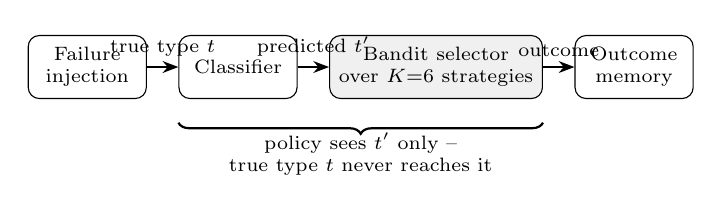
\begin{tikzpicture}[
  node distance = 4mm and 4mm,
  box/.style = {draw, rounded corners, minimum height=8mm, minimum width=15mm,
                align=center, font=\scriptsize},
  arr/.style = {-{Stealth[length=2mm]}, thick}
]
  \node[box] (inj) {Failure\\injection};
  \node[box, right=of inj] (clf) {Classifier};
  \node[box, right=of clf, fill=gray!12] (sel) {Bandit selector\\over $K{=}6$ strategies};
  \node[box, right=of sel] (mem) {Outcome\\memory};

  \draw[arr] (inj) -- (clf) node[midway, above, font=\scriptsize] {true type $t$};
  \draw[arr] (clf) -- (sel) node[midway, above, font=\scriptsize] {predicted $t'$};
  \draw[arr] (sel) -- (mem) node[midway, above, font=\scriptsize] {outcome};

  \draw[decorate, decoration={brace, amplitude=4pt, mirror}, thick]
       ($(clf.south west)+(0,-3mm)$) -- ($(sel.south east)+(0,-3mm)$)
       node[midway, below, font=\scriptsize, align=center]
       {policy sees $t'$ only --\\true type $t$ never reaches it};
\end{tikzpicture}
\caption{Position of the classifier in the decision path. Policies observe
only the predicted type $t'$, never the true type $t$; this is the
structural fact that motivates the extension in Section~\ref{sec:method}.}
\label{fig:framework}
\end{figure}

\section{Problem Statement}

Let $\mathrm{confusion}[t,t'] = \Pr(\text{predicted } t' \mid \text{true }
t)$ describe the classifier. The base predictor implicitly assumes
$\mathrm{confusion} = I$. Ours does not, and that leaves two open
questions. First: what is the correct crossover prediction once the
policy conditions on $t'$ instead of $t$? This has an exact answer on the
static side and only an approximate one on the adaptive side. Second:
does a free constant fitted under one classifier condition transfer to
another? If a $\kappa$ fitted on perfect-classifier data predicts
noisy-classifier held-out cells about as well as a $\kappa$ fitted
directly on noisy-classifier data, the reformulation has absorbed the
classifier effect and whatever error is left over is inherited from the
base bound. If not, the reformulation is introducing error of its own.
Telling these apart needs genuinely held-out data and a decision rule
fixed before looking, for reasons we come back to in
Section~\ref{sec:setup}.

\section{Proposed Methodology}
\label{sec:method}

\subsection{The effective mixture matrix}

Marginalising over true types gives the predicted-type distribution
\begin{equation}
p'[t'] = \sum_t p[t] \cdot \mathrm{confusion}[t,t']. \label{eq:marginal}
\end{equation}
Applying Bayes' rule inside each predicted bucket gives the effective
success probability of strategy $k$ given that the classifier predicted
$t'$:
\begin{equation}
P_{\mathrm{eff}}[t',k] = \frac{\sum_t p[t]\,\mathrm{confusion}[t,t']\,P[t,k]}{p'[t']}. \label{eq:peff}
\end{equation}
Both are exact, with no approximation at this stage, and collapse to $p'
= p$ and $P_{\mathrm{eff}} = P$ when $\mathrm{confusion} = I$.
$P_{\mathrm{eff}}$ is the central object of the extension: given that the
classifier said $t'$, how well does strategy $k$ actually work, averaged
over what the type really was.

\subsection{Static and adaptive sides under confusion}

The static side follows by composing two existing exact functions:
\begin{equation}
\rho_{\mathrm{conf}} = \mathrm{oracle}(P,p) - \mathrm{policy}_{\mathrm{conf}}(P,\pi,\mathrm{confusion},p), \label{eq:rhoconf}
\end{equation}
which is exact, not asymptotic. The adaptive side reuses the base bound
unmodified, evaluated on the mixture instead of the true matrix:
\begin{equation}
R^{\mathrm{conf}}_{\mathrm{TS}}(T) = R_{\mathrm{TS}}(P_{\mathrm{eff}}, T, N, p', \mathrm{form}, \kappa). \label{eq:rtsconf}
\end{equation}
The crossover horizon under confusion solves
\begin{equation}
R^{\mathrm{conf}}_{\mathrm{TS}}(T) = \rho_{\mathrm{conf}} \cdot T. \label{eq:crossoverconf}
\end{equation}
We implemented Eq.~(\ref{eq:crossoverconf}) as its own routine rather
than a thin wrapper on the base solver, since it mixes index spaces:
$\rho_{\mathrm{conf}}$ lives in true-type space while the regret term
lives in predicted-type space, and the base solver always computes its
own $\rho$ from the same triple that feeds the regret term, so it cannot
represent this combination. The numerical method (a unimodal scan
followed by bracketing refinement) is shared code, and at
$\mathrm{confusion} = I$ unit tests confirm the extension returns
bit-for-bit what the base solver returns, so this is a strict
generalisation, not a parallel reimplementation that happens to agree.

We also report a ceiling reduction,
\begin{equation}
\Delta_{\mathrm{ceil}} = \mathrm{oracle}(P,p) - \mathrm{oracle}(P_{\mathrm{eff}}, p'), \label{eq:ceiling}
\end{equation}
exact, provably non-negative, and zero exactly when $\mathrm{confusion} =
I$. Of the extension's pieces, the effective matrix, $\rho_{\mathrm{conf}}$,
the ceiling reduction, the gap-shrinkage report, and the argmax-inversion
check are all exact; only $R^{\mathrm{conf}}_{\mathrm{TS}}$ and the
crossover horizon itself inherit the base predictor's asymptotic
approximation. That split feels like a more honest way to describe the
contribution than calling it a new bound: exact machinery built around an
existing asymptotic one, with a clear record of which part is which.

\subsection{Assumptions}

Five assumptions carry this extension, stated with their actual status
rather than as if all were equally safe. A1 (predicted-type bucket
structure) is verified at the implementation level by tracing the call
chain, not assumed from documentation. A2 (conditionally Bernoulli
rewards) is inherited unchanged. A3 (stationary confusion matrix) rules
out classifier drift within the analysed horizon, optimistic if the
classifier itself gets worse over time. A4 (the asymptotic regret bound)
holds as $T \to \infty$, not at finite time, and still carries the
uncalibrated $\kappa$. A5 (scalar accuracy as a stand-in for a full
confusion matrix) is a real simplification, one we mostly avoid by
validating against the trained classifier's actual, non-uniform matrix.

\subsection{Two channels of degradation, and two sanity checks}

Classifier noise hurts in two distinguishable ways: merging true types
into indistinguishable predicted buckets destroys information and lowers
the achievable reward ceiling regardless of policy (Eq.~\ref{eq:ceiling}),
while separately changing the gap between the best and second-best action
inside each predicted bucket, which changes how hard the
arm-identification problem is. The first is a ceiling effect, the second
a learnability effect, and nothing forces them to move together.

Could a predicted bucket's best action under $P_{\mathrm{eff}}$ turn out
optimal for none of the true types feeding it, recommending something no
constituent type actually wanted? It does not happen at our classifier's
measured confusion (Section~\ref{sec:results}), and a small constructed
three-type counter-example confirms the check fires when its structural
condition holds: two comparably weighted contributors with different
argmaxes and no single dominant one.

Separately, $\rho$ and the ceiling reduction are provably monotonic in
classifier accuracy, but $T^*$ is not. A small two-type, two-strategy
unit test has a predicted bucket whose best arm changes identity as
accuracy crosses a threshold, making that bucket's top-two gap V-shaped:
large at both ends, zero at the flip, regardless of $\kappa$. This rules
out the tempting inference that a somewhat better classifier implies a
somewhat earlier crossover.

\section{Experimental Setup}
\label{sec:setup}

An earlier pass at this validation fitted $\kappa$ and evaluated it on
the same three environments, since only three existed at the time. Those
numbers are not really validation: a low error drawn from the same
three-cell subset used for fitting is indistinguishable from tuning to
those points. That analysis is still in version control for transparency
but no longer reported as a result. Fixing it needed a real split and a
protocol committed before new data existed.

A read-only forensic check found the committed sweep table had only ever
held 3 of the intended 26 environments; we loaded all 617 files in the
sweep result store rather than sampling them, and the missing 23 had no
trace anywhere, a genuine never-simulated gap traced back to a stale
status note, not a lost cache or a filtering bug. Closing it meant new
simulation, filtered to the two methods the primary analysis needs
(static baseline, Thompson sampling): a 312-cell grid, 26 environments
$\times$ 2 classifier conditions $\times$ 2 methods $\times$ 3 seeds, 204
of them new, giving 26 environments $\times$ 2 conditions, 52 cells,
2{,}184 rows across 7 horizons.

The protocol itself was written and committed before that 26-environment
data existed:

\begin{itemize}
\setlength\itemsep{1pt}
\setlength\parskip{0pt}
\item \textbf{Split.} Of the 25 gap-family environments, 8 went to TEST by
a fixed-seed draw (seed 19001). The one non-gap-family environment stayed
in TRAIN unconditionally, since holding out its only family member would
test a different question. That gives 18 TRAIN and 8 TEST. Two
environments already known from the superseded analysis to have poor
errors happened to land in TEST; we did not redraw the seed once that was
seen.
\item \textbf{Fitting.} Bounded 1-D least squares minimising mean squared
log-space error, bounds $(\log 10^{-3}, \log 10^{4})$, KL form fixed, the
same procedure the base predictor itself uses.
\item \textbf{Branches.} Branch A, transfer: fit $\kappa_A$ on TRAIN
perfect-classifier cells and apply it unchanged to TEST noisy-classifier
cells. Branch B, in-condition: fit $\kappa_B$ on TRAIN noisy-classifier
cells and apply it to the same TEST cells, the best achievable
same-condition benchmark.
\item \textbf{Decision rule.} $R = E_A/E_B$, median absolute relative
error. $R \le 1.5$ was pre-committed to Case 1, the effect is absorbed
and residual error is inherited; $R > 1.5$ to Case 2, the extension adds
error of its own, reported with no rescue attempt. The threshold of 1.5
is a disclosed judgment call, roughly midway between a too-lenient factor
of three and a too-strict factor of one.
\item \textbf{Power floor.} Fewer than 5 finite cells in either branch
means no Case 1 or Case 2 conclusion, reported instead as underpowered.
\item \textbf{Uncertainty.} Environment-level bootstrap, seed 19002,
2{,}000 resamples: held-out error uncertainty by resampling TEST
environments and reusing the fitted constants, and fit uncertainty by
resampling TRAIN environments and refitting per branch.
\item \textbf{Naming rule.} A fitted constant within one order of
magnitude of the base predictor's own best fit, $[0.00045, 0.045]$, would
be called a calibrated predictor rather than a validated bound. This was
decided before the fitted value was seen.
\item \textbf{Commitment.} One specification, no second attempt: no other
split, form, threshold, or bound would be tried after seeing results.
\end{itemize}

Simulations ran on an Intel Core i5-9300H CPU (4 physical cores, 8
logical processors, 2.40\,GHz) with 8\,GB RAM under Windows 11 Home
Single Language (build 10.0.26200, 64-bit), using CPython 3.13.11 with
NumPy 2.5.1, pandas 3.0.3, SciPy 1.18.0, and scikit-learn 1.9.0. Parallel
execution used a process-based backend (\texttt{joblib}, \texttt{loky})
with a content-addressed result store, so interrupted runs could resume.

\section{Results and Discussion}
\label{sec:results}

\subsection{Two-channel decomposition at the real classifier}

At the trained classifier's empirical confusion matrix, mean diagonal
accuracy 0.939 (Fig.~\ref{fig:confusion}), the ceiling reduction is 0.0120
and the mean gap shrinkage across the seven predicted buckets is 0.0020.
Ceiling loss runs about six times larger than learnability loss at this
accuracy. Both are real and neither is zero, but most of the measured
degradation looks like information destroyed by merging types, not a
harder arm-identification problem. That split is specific to this
classifier's confusion structure and should not be treated as a general
ratio. The argmax-inversion check does not fire in any of the seven
predicted buckets here.

\begin{figure}[t]
\centering
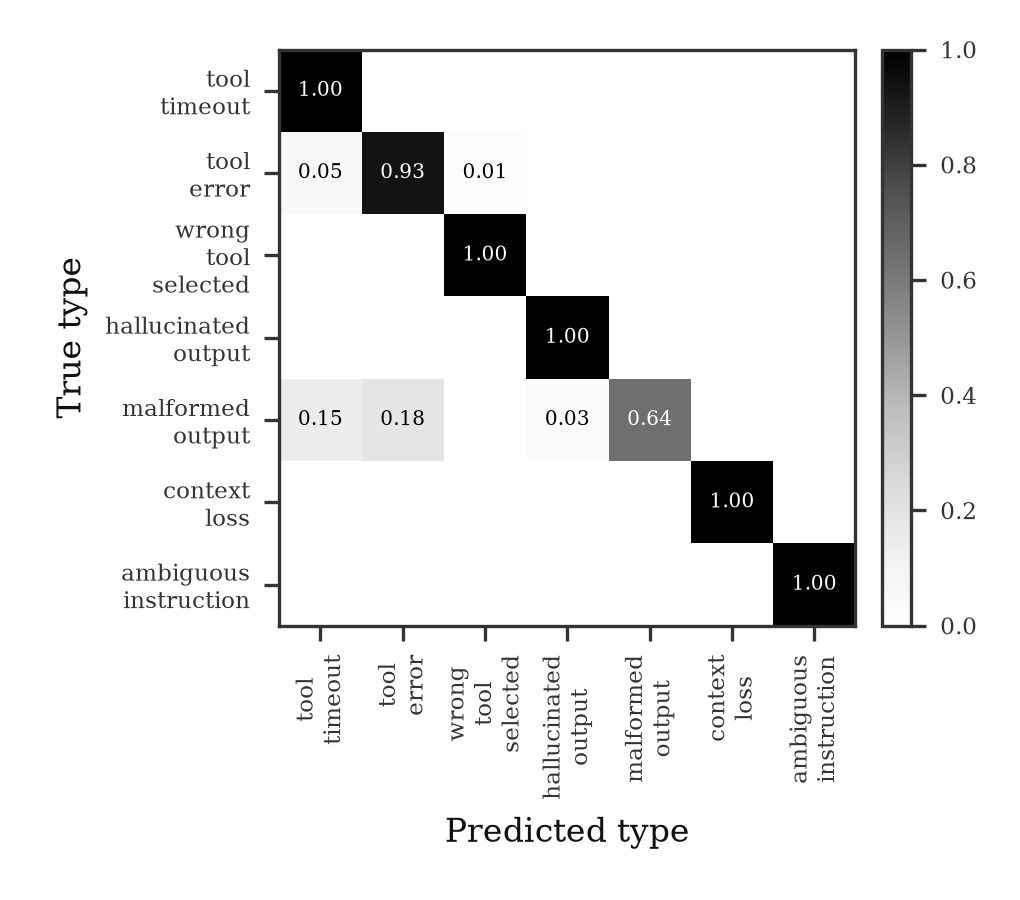
\includegraphics[width=0.68\linewidth]{fig2_confusion_matrix.png}
\caption{Empirical confusion matrix of the trained classifier,
$P(\text{predicted}\mid\text{true})$, mean diagonal accuracy 0.939.
Confusion is concentrated almost entirely in one row
(\texttt{malformed\_output}), which is most of why the ceiling and
learnability losses above are not spread evenly across predicted
buckets.}
\label{fig:confusion}
\end{figure}

\subsection{Static-side validation}

We checked the exact static component of Eq.~(\ref{eq:rhoconf}) against
an existing table of six noise levels with 50 already-simulated seeds
each. That table has no adaptive-method trajectory in it, so it validates
the static side only; it is never used as evidence for the adaptive
theory. Results are in Table~\ref{tab:static}. A median absolute error of
0.93 percentage points is the strongest validation result anywhere in
this work, which is about what one would expect from a component that is
exact closed-form arithmetic rather than an asymptotic approximation.

\begin{table}[t]
\centering
\caption{Static-side validation. Predicted versus empirical per-episode
rate across noise levels $\beta$; 50 seeds per level.}
\label{tab:static}
\footnotesize
\begin{tabular}{cccc}
\hline
$\beta$ & Predicted & Empirical & Abs. error \\
\hline
0.0 & 0.4408 & 0.4306 & 0.0102 \\
0.1 & 0.4691 & 0.4582 & 0.0109 \\
0.3 & 0.5256 & 0.5112 & 0.0144 \\
0.5 & 0.5821 & 0.5744 & 0.0077 \\
0.8 & 0.6669 & 0.6584 & 0.0085 \\
1.0 & 0.7234 & 0.7156 & 0.0078 \\
\hline
\multicolumn{3}{l}{Median absolute error} & \textbf{0.0093} \\
\hline
\end{tabular}
\end{table}

\subsection{Held-out evaluation of the free constant}

The power check cleared with room to spare: 18 of 18 TRAIN cells and 8 of
8 TEST cells were finite in both branches, against a floor of 5. Headline
results sit in Table~\ref{tab:kappa}.

\begin{table}[t]
\centering
\caption{Pre-registered held-out evaluation. Errors are median absolute
relative error on the eight held-out TEST cells.}
\label{tab:kappa}
\footnotesize
\begin{tabular}{lcc}
\hline
 & \textbf{Branch A} & \textbf{Branch B} \\
 & (transfer) & (in-condition) \\
\hline
Fitted constant & 0.044381 & 0.042559 \\
TRAIN cells used & 18 & 18 \\
Held-out error & 59.7\% & 40.5\% \\
Fit 95\% CI & [0.0369, 0.0544] & [0.0105, 0.0426] \\
\hline
\multicolumn{3}{l}{$R = E_A/E_B = 0.5970/0.4053 = \mathbf{1.4729}$} \\
\multicolumn{3}{l}{Threshold 1.5; margin 1.8\%} \\
\multicolumn{3}{l}{Bootstrap 95\% CI for $R$: $[1.00,\ 9.55]$} \\
\hline
\end{tabular}
\end{table}

The point estimate satisfies the pre-committed rule, so this is a Case 1
outcome: the mixture reformulation captures the classifier-noise effect,
and the prediction error left over is inherited asymptotic-bound bias
rather than something this extension introduced. Two things temper that.
Absolute errors of 59.7\% and 40.5\% are still large, and the base bound
is not suddenly more accurate because of this result; what the test
actually shows is a pre-existing limitation transferring cleanly, not
being resolved.

The margin is thin, just 1.8\%, and the pre-registered bootstrap interval
for $R$ runs all the way to 9.55, nearly 6.4$\times$ past the threshold
and well into Case 2 territory. That interval was required by the
protocol, not optional colour, and a different draw of held-out
environments could plausibly have landed in Case 2 instead. The
fit-uncertainty bootstrap tells a consistent story: the noisy-condition
fit is markedly less stable than the transferred one.

Table~\ref{tab:percell} and Fig.~\ref{fig:percell} show why the medians
above should not be read as a tight summary. Errors are heterogeneous.
Two environments over-predict by roughly 5.75$\times$ under both
constants, and one under-predicts by roughly 3$\times$. No single scalar
constant fixes this spread, and in keeping with the protocol's no-rescue
commitment, we did not try to introduce one.

\begin{table}[t]
\centering
\caption{Branch A per-cell results on the eight held-out TEST
environments.}
\label{tab:percell}
\footnotesize
\begin{tabular}{lcc}
\hline
\textbf{Environment} & \textbf{Ratio} & \textbf{Signed rel. error} \\
\hline
gap0.20\_idx00 & 1.487 & +48.7\% \\
gap0.20\_idx01 & 1.527 & +52.7\% \\
gap0.20\_idx06 & 1.283 & +28.3\% \\
gap0.20\_idx08 & 5.756 & +475.6\% \\
gap0.20\_idx11 & 0.675 & $-32.5\%$ \\
gap0.20\_idx16 & 0.333 & $-66.7\%$ \\
gap0.20\_idx17 & 5.752 & +475.2\% \\
gap0.20\_idx24 & 1.694 & +69.4\% \\
\hline
\end{tabular}
\end{table}

\begin{figure}[t]
\centering
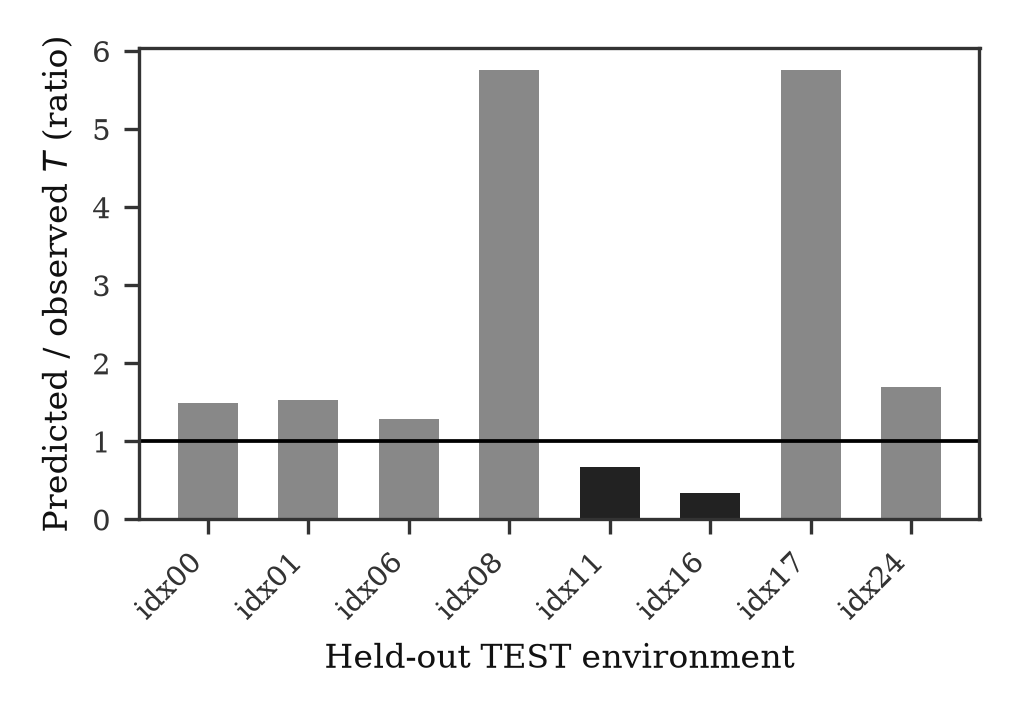
\includegraphics[width=0.68\linewidth]{fig4_percell_heldout.png}
\caption{Branch A predicted/observed ratio for each of the eight held-out
TEST environments. A ratio of 1 (solid line) is a perfect prediction;
black bars under-predict, grey bars over-predict. Two environments
(\texttt{idx08}, \texttt{idx17}) over-predict by more than 5$\times$,
which is most of why the median looks tighter than the actual spread.}
\label{fig:percell}
\end{figure}

The fitted transfer constant, 0.0444, sits inside the pre-committed
calibrated-predictor range, near its upper edge. We describe this
component as a calibrated predictor with theoretical motivation, not a
validated bound.

\subsection{Classification}

We classify the crossover extension as partially supported: neither
validated nor unvalidated. Case 1 is the pre-committed outcome and real
held-out evidence for the first time in this line of work, a genuine step
up from the superseded in-sample analysis, but the fragility is just as
real. The result meets the pre-registered criterion without meeting it
robustly, which is why we use a three-tier vocabulary instead of a
two-tier one that would round this up to ``validated.''
Table~\ref{tab:classification} lists every component's status.

\begin{table}[t]
\centering
\caption{Component classification.}
\label{tab:classification}
\footnotesize
\begin{tabular}{ll}
\hline
\textbf{Component} & \textbf{Status} \\
\hline
Effective matrix, Eq.~(\ref{eq:marginal})--(\ref{eq:peff}) & Validated \\
$\rho_{\mathrm{conf}}$, Eq.~(\ref{eq:rhoconf}) & Validated \\
Ceiling reduction, Eq.~(\ref{eq:ceiling}) & Validated \\
Gap-shrinkage report & Validated \\
Argmax-inversion check & Validated \\
$T^*$ non-monotonicity & Validated (shape finding) \\
$R^{\mathrm{conf}}_{\mathrm{TS}}$, Eq.~(\ref{eq:rtsconf}) & Partially supported \\
Crossover horizon / $\kappa$ & Partially supported \\
Drift sign rule (Sec.~\ref{sec:drift}) & Negative result \\
\hline
\end{tabular}
\end{table}

\subsection{Drift: a documented negative result}
\label{sec:drift}

A separate extension asks whether a low-dimensional summary statistic can
predict the sign of adaptive advantage under environment drift, out of
sample. The two extensions do not depend on each other; their assumption
numbering is even kept separate on purpose. We fixed the falsifiable
structure before trying anything: a candidate statistic has to beat a
majority-class guess under leave-one-cell-out evaluation. Three
candidates were pre-registered and tried in order, with a fourth ruled
out in advance if the third failed. The substrate is a dense
pre-simulated grid of 12{,}800 cells across four drift mechanisms.

Table~\ref{tab:drift} and Fig.~\ref{fig:driftattempts} summarise what
happened. We retracted the second attempt before it could be reported as
a finding, because its recovery-ratio term has the base predictor sitting
in its own denominator. Testing whether that term predicts adaptive
advantage was mostly testing whether the base bound has some validity,
applied row by row, which is not independent confirmation of anything
new. There was no statistical circularity here, but the conceptual
circularity was real and it mattered.

\begin{table}[t]
\centering
\caption{Three pre-registered attempts at a quantitative sign rule under
drift.}
\label{tab:drift}
\footnotesize
\begin{tabular}{cll}
\hline
\textbf{\#} & \textbf{Statistic} & \textbf{Outcome} \\
\hline
1 & survival, gap-change & $R^2=0.012$; insufficient \\
2 & magnitude, recovery-ratio & $R^2=0.579$--$0.735$; retracted \\
3 & env. regret, reversion & $R^2=0.676$; sign acc. \\
  & & $79.7\%$ = majority baseline \\
\hline
\end{tabular}
\end{table}

\begin{figure}[t]
\centering
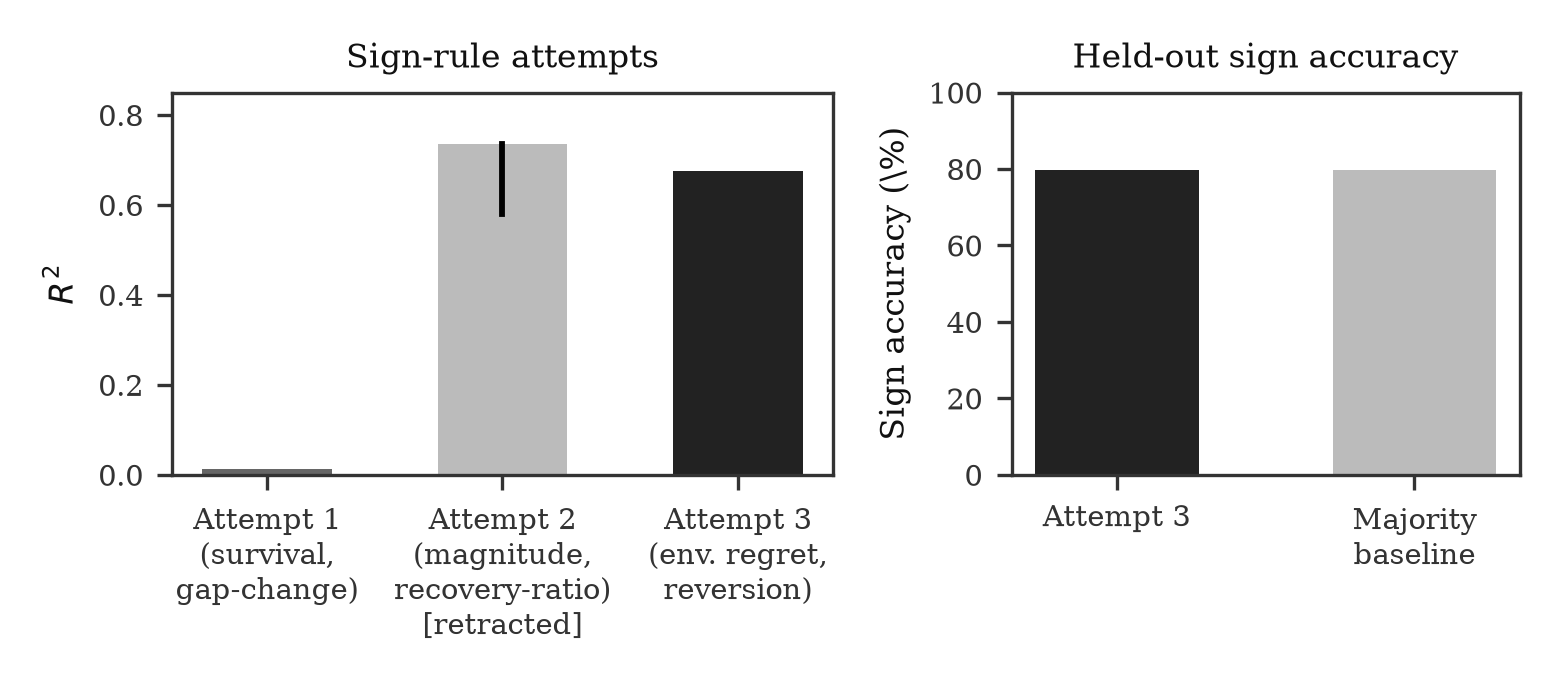
\includegraphics[width=0.78\linewidth]{fig5_drift_attempts.png}
\caption{Left: $R^2$ for the three pre-registered sign-rule attempts
(Attempt 2's bar spans its reported range; it was retracted before
counting as a finding). Right: Attempt 3's held-out sign accuracy against
the majority-class baseline it needed to beat. The two bars come out
equal, which is the negative result in one picture.}
\label{fig:driftattempts}
\end{figure}

A methodological wrinkle turned up along the way: the first-attempt
statistics were computed as means over touched rows only, blind to how
many of an environment's rows were actually touched. Most of what looked
like magnitude's contribution in the second attempt ($+0.156\ R^2$) was
an artifact of that exclusion, since recomputing at the environment level
shrank the apparent gain to $+0.006$ (checked against an existing
regret-rate function to $2.78 \times 10^{-16}$ as a construction-identity
test, never used predictively). The lesson: a statistic at the wrong
aggregation level can look like it needs an extra variable when it does
not, and the fix is recomputing it, not patching one in.

One finding does survive on its own, separate from the failed
quantitative rules: the sign of adaptive advantage under drift is
governed by whether staleness damage reverts, not by how large it is. All
13 negative-advantage cells sit at a reversion fraction of at least 0.68
across 260 seed draws; all 32 cells with reversion near zero come out
positive across 640 draws. Monotone-decay's reversion fraction sits near
zero with a precise 95\% interval, $[0.0000, 0.0160]$ at $n=236$, small
sample and all, which we treat as part of the finding rather than hide in
a footnote. This pattern holds up even though no quantitative threshold
built on it survives out-of-sample testing, and it also explains
something that had puzzled us: the static table beats the adaptive
learner in 10 of 16 partial-reorder cells, because best/second-best swaps
revert on a period-2 cycle there, so the static table's stale action
stays near-optimal while the learner keeps paying exploration cost
chasing a target that drifts back to where it already was. We treat this
as correlational with a mechanism behind it, not causal; the mechanism
was designed before this analysis and never varied independently, and a
real causal test would need drift processes matched on damage magnitude
with reversion varied on its own, which we did not run.

Drift-type fixed effects still retain $+0.092\ R^2$ beyond the
two-statistic summary, genuine structure we have not accounted for.
Having committed to stopping at three attempts we did not chase it
further, though disruption abruptness, within-row breadth, and available
recovery time relative to shift frequency all look like plausible
candidates. The sign of adaptive advantage under drift does not reduce to
a two-statistic summary across these four regimes, at least given the
data and methods available here.

\section{Reproducibility and Measurement Findings}

Estimating the cost of the sweep in Section~\ref{sec:setup} taught us
more than we expected about our own tooling, and since it undercuts cost
figures we published elsewhere in this project, we report it here rather
than bury it in an appendix. The sweep script's cost estimator assumes
linear parallel speedup when dividing single-threaded throughput by
worker count, an assumption stated in its own docstring and untrue on our
hardware. Table~\ref{tab:estimate} shows the reconciliation: 38.4 minutes
projected against roughly 81.9 actual, about $2.13\times$ over, matching
an earlier rate check that had already flagged a $2.3\times$ miss.

We first suspected BLAS thread oversubscription, tested it by reading
the thread-pool state from inside a worker process, and found it false;
the parallel backend already pins one thread per worker on its own. We
retracted that hypothesis immediately, though the underlying defect
stands: a four-physical-core machine under hyperthreading explains the
gap well enough by itself. Two separate measurements of effective
parallelism, about 45 minutes apart on the same workload, disagreed by
roughly 44\% ($1.90\times$ versus $2.74\times$); we report that as an
open finding rather than average it away, with concurrent foreground load
during the first window as the likeliest, unconfirmed, cause. One
stop-rule also got misapplied mid-run, a threshold meant for a bad
\emph{estimate} was applied to a genuine \emph{measurement}, killing a
run unnecessarily before we caught the mistake. This project's own
published sweep-cost figures elsewhere, roughly 73 and 66 hours for two
full-scale runs, rest on the same false assumption and have not been
re-derived; we flag them as suspect rather than fix them here. Full
incident detail lives in the project repository.

\begin{table}[t]
\centering
\caption{Estimated versus actual wall-clock for the filtered 204-cell
sweep.}
\label{tab:estimate}
\footnotesize
\begin{tabular}{lc}
\hline
Original estimate & 38.4 min \\
Actual total (two attempts) & $\approx 81.9$ min \\
Ratio & $\approx 2.13\times$ \\
Consistent with early-rate check ($\approx 2.3\times$)? & Yes \\
\hline
\end{tabular}
\end{table}

\section{Limitations}

Scope is the most restrictive limitation here. The held-out evaluation
covers one matrix family at a single gap level, so generalisation across
other gap structures and environment families is untested, and eight
held-out environments is a small test set whose spread
(Table~\ref{tab:percell}) shows the median is not a tight summary. The
adaptive-side result is a point estimate that clears its threshold by
only 1.8\%, with a bootstrap interval spanning $[1.00, 9.55]$; we think
the interval is the more informative number and have tried not to let the
favourable point estimate carry more weight than it can bear.

The extension also inherits every limitation the base bound already had:
asymptotic rather than finite-time, an empirically fitted constant, and
reliable only in a narrow regime, so absolute held-out errors near 40 and
60 percent should be read with that in mind. Assumption A3 rules out
classifier drift within the analysed horizon, optimistic for any
deployment where the classifier itself degrades, and A5's
scalar-accuracy shortcut is a real simplification only partly offset by
validating against the actual confusion matrix.

On the drift side, the surviving positive finding is correlational with
a mechanism behind it, not causal, and that mechanism was never varied
independently; the $+0.092\ R^2$ of drift-type structure remains
unexplained. Finally, the cost figures reported elsewhere in this project
rest on an assumption now known false and have not been re-derived, and
timing numbers collected before the hygiene protocol was adopted have
conditions we can no longer fully specify.

\section{Conclusion and Future Work}

We extended a crossover-horizon predictor to the setting our system
actually lives in, where recovery policies see a classifier's prediction
rather than the true failure type. The extension is exact where it can
be, collapses identically to its predecessor at a perfect classifier, and
splits classifier-induced degradation into a ceiling channel and a
learnability channel, the former about six times the latter at our
classifier's measured accuracy, and showed the predicted horizon is not
monotonic in accuracy, ruling out an intuitive design heuristic.

The free constant was evaluated under a protocol fixed before the data
existed: the pre-registered criterion is satisfied by point estimate, the
same protocol's own uncertainty quantification does not confirm that
satisfaction is robust, and we call the component a calibrated predictor
rather than a validated bound. The companion drift investigation produced
no quantitative sign rule and stands as a negative result, with one
qualitative finding that survives.

A few directions follow from here: extending the held-out evaluation to
independently generated environment families at multiple gap levels;
relaxing the stationary-confusion assumption so the two extensions
connect instead of staying independent; a genuinely causal drift test
with damage magnitude matched and reversion varied on its own; and
re-deriving this project's cost figures from measured rather than assumed
parallelism.

\section*{Acknowledgment}

I thank my project supervisor, Ms. Divina, for her guidance and feedback
throughout this work.

\begin{thebibliography}{10}

\bibitem{lai1985}
T.~L. Lai and H.~Robbins, ``Asymptotically efficient adaptive allocation
rules,'' \emph{Advances in Applied Mathematics}, vol.~6, no.~1, pp.
4--22, Mar. 1985, doi: 10.1016/0196-8858(85)90002-8.

\bibitem{auer2002}
P.~Auer, N.~Cesa-Bianchi, and P.~Fischer, ``Finite-time analysis of the
multiarmed bandit problem,'' \emph{Machine Learning}, vol.~47, no.~2--3,
pp. 235--256, 2002, doi: 10.1023/A:1013689704352.

\bibitem{thompson1933}
W.~R. Thompson, ``On the likelihood that one unknown probability exceeds
another in view of the evidence of two samples,'' \emph{Biometrika},
vol.~25, no.~3--4, pp. 285--294, Dec. 1933, doi: 10.1093/biomet/25.3-4.285.

\bibitem{russo2018}
D.~J. Russo, B.~Van Roy, A.~Kazerouni, I.~Osband, and Z.~Wen, ``A
tutorial on Thompson sampling,'' \emph{Foundations and Trends in Machine
Learning}, vol.~11, no.~1, pp. 1--96, 2018, doi: 10.1561/2200000070.

\bibitem{shinn2023}
N.~Shinn, F.~Cassano, E.~Berman, A.~Gopinath, K.~Narasimhan, and S.~Yao,
``Reflexion: Language agents with verbal reinforcement learning,'' in
\emph{Advances in Neural Information Processing Systems 36 (NeurIPS
2023)}, 2023, arXiv:2303.11366.

\bibitem{gou2024}
Z.~Gou, Z.~Shao, Y.~Gong, Y.~Shen, Y.~Yang, N.~Duan, and W.~Chen,
``CRITIC: Large language models can self-correct with tool-interactive
critiquing,'' in \emph{Proc. 12th International Conference on Learning
Representations (ICLR)}, 2024, arXiv:2305.11738.

\bibitem{cemri2025}
M.~Cemri, M.~Z. Pan, S.~Yang, L.~A. Agrawal, B.~Chopra, R.~Tiwari,
K.~Keutzer, A.~G. Parameswaran, D.~Klein, K.~Ramchandran, M.~Zaharia,
J.~E. Gonzalez, and I.~Stoica, ``Why do multi-agent LLM systems fail?,''
arXiv:2503.13657, 2025, doi: 10.48550/arXiv.2503.13657.

\bibitem{zhu2025}
K.~Zhu, Z.~Liu, B.~Li, M.~Tian, Y.~Yang, J.~Zhang, P.~Han, Q.~Xie,
F.~Cui, W.~Zhang, X.~Ma, X.~Yu, G.~Ramesh, J.~Wu, Z.~Liu, P.~Lu, J.~Zou,
and J.~You, ``Where LLM agents fail and how they can learn from
failures,'' arXiv:2509.25370, 2025.

\bibitem{vuddanti2025}
S.~V. Vuddanti, A.~Shah, S.~K. Chittiprolu, T.~Song, S.~Dev, K.~Zhu, and
M.~Chaudhary, ``PALADIN: Self-correcting language model agents to cure
tool-failure cases,'' arXiv:2509.25238, 2025.

\bibitem{song2025aegis}
K.~Song, A.~Jayarajan, Y.~Ding, Q.~Su, Z.~Zhu, S.~Liu, and G.~Pekhimenko,
``Aegis: Taxonomy and optimizations for overcoming agent-environment
failures in LLM agents,'' arXiv:2508.19504, 2025.

\end{thebibliography}

\end{document}
